\section{Processes}

\paragraph{The Process Abstraction}
\begin{itemize}
	\item computers do "`several things at the same time"' (just looks this way though quick process switching (\textbf{Multiprogramming}))
	\item \( \leadsto \) \textbf{process} abstraction models this concurrency: \\*
		- container contains information about program execution \\*
		- conceptually, every progress has own "`virtual CPU"' \\*
		- execution context is changed on process switch \\*
		- dispatcher switches context when switching processes \\*
		- \textbf{context switch}: dispatcher saves current registers/memory \\* \phantom{-} mappings, restores those of next process
\end{itemize}

\paragraph{Process-Cooking Analogy}
\begin{itemize}
	\item Program/Process like Recipe/Cooking
	\item \textbf{Recipe}: lists ingredients, gives algorithm what to do when \\*
		\( \leadsto \) program describes memory layout/CPU instructions
	\item \textbf{Cooking}: activity of using the recipe \\*
		\( \leadsto \) process is activity of executing a program
	\item multiple similar recipes for same dish \\*
		\( \leadsto \) multiple programs may solve same problem
	\item recipe can be cooked in different kitchens at the same time \\*
		\( \leadsto \) program can be run on different CPUs at the same time \\* \phantom{\( \leadsto \)} (as different processes)
	\item multiple people can cook one recipe \\*
		\( \leadsto \) one process can have several worker threads
\end{itemize}

\paragraph{Concurrency vs. Parallelism}
\begin{itemize}
	\item OS uses currency + parallelism to implement multiprogramming
	\begin{enumerate}
		\item \textbf{Concurrency}: multiple processes, one CPU \\* \( \leadsto \) not at the same time
		\item \textbf{Parallelism}: multiple processes, multiple CPU \\* \( \leadsto \) at the same time
	\end{enumerate}
\end{itemize}

\paragraph{Virtual Memory Abstraction --- Address Spaces}
\begin{itemize}
	\item every process has own \emph{virtual addresses} (vaddr)
	\item MMU relocates each load/store to \emph{physical memory} (pmem)
	\item processes never see physical memory, can't access it directly
	\item \textcolor{black!60!green}{\code{+}} MMU can enforce protection (mappings in kernel mode)
	\item \textcolor{black!60!green}{\code{+}} programs can see more memory than available \\*
		\phantom{x} 80:20 rule: 80\% of process memory idle, 20\% active \\*
		\phantom{x} can keep working set in RAM, rest on disk
	\item \textcolor{red}{\code{-}} need special MMU hardware
\end{itemize}

\paragraph{Address Space (Process View)}
\begin{itemize}
	\item code/data/state need to be organized within process \\*
		\( \leadsto \) \textbf{address space layout}
	\item Data types:
	\begin{enumerate}
		\item \emph{fixed size} data items
		\item data naturally \emph{freed in reverse allocation order}
		\item data \emph{allocated/freed "`randomly"'}
	\end{enumerate}
	\item compiler/architecture determine how large int is and what instructions are used in text section (\code{code})
	\item \textbf{Loader} determines based on exe file how executed program is placed in memory
\end{itemize}

\paragraph{Segments --- Fixed-Size Data + Code}
\begin{itemize}
	\item some data in programs never changes or will be written but never grows/shrinks \\*
		\( \leadsto \) memory can be statically allocated on process creation
	\item \textbf{BSS segment} (\emph{block started by symbol}): \\*
		- statically allocated variables/non-initialized variables \\*
		- executable file typically contains starting address + size of BSS \\*
		- entire segment initially 0
	\item \textbf{Data segment}: \\*
		- fixed-size, initialized data elements (e.g. global variables)
	\item \textbf{read-only data segment}: \\*
		- constant numbers, strings
	\item All three sometimes summarized as one segment
	\item compiler and OS decide ultimately where to place which data/how many segments exist
\end{itemize}

\paragraph{Segments --- Stack}
\begin{itemize}
	\item some data naturally freed in reverse allocation order \\*
		\( \leadsto \) very easy memory management (stack grows upwards)
	\item fixed segment starting point
	\item store top of latest allocation in \textbf{stack pointer} (SP) \\*
		(initialized to starting point)
	\item \emph{allocate} \code{a} byte data structure: \code{SP += a; return(SP - a)}
	\item \emph{free} \code{a} byte data structure: \code{SP -= a}
\end{itemize}

\paragraph{Segments --- Heap (Dynamic Memory Allocation)}
\begin{itemize}
	\item some data "`randomly"' allocated/freed
	\item two-tier memory allocation:
	\begin{enumerate}
		\item allocate large memory chunk (\textbf{heap segment}) from OS \\*
			- base address + \textbf{break pointer} (BRK) \\*
			- process can get more/give back memory from/to OS \\*
		\item dynamically partition chunk into smaller allocations \\*
			- \code{malloc}/\code{free} can be used in random oder \\*
			- purely user-space, no need to contact kernel
	\end{enumerate}
\end{itemize}

\begin{figure}[h]\centering\label{AddressSpaceLayoutComplex}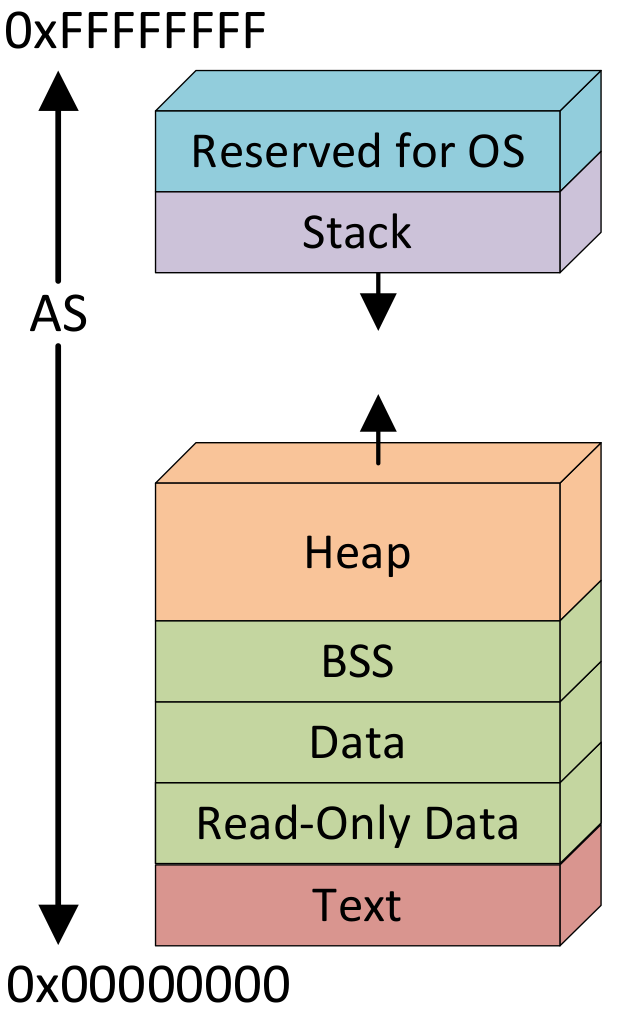
\includegraphics[width=0.2\textwidth]{AddressSpaceLayoutComplex}\end{figure}

\begin{summary}
	\begin{itemize}
		\item recipe vs. cooking is like program vs. process
		\item processes = resource container for OS
		\item process feels alone: has own CPU + memory
		\item OS implements multiprogramming through rapid process switching
	\end{itemize}
\end{summary}